\section{A Data Type for Analytic Functions}
\subsection{Analytic Functions}
\begin{frame}
\frametitle{Analytic Functions and Computational Complexity}
\begin{fact}
For general polynomial time computable functions, many important operators have been shown to be computationally hard.\\
For example
\begin{itemize}[<+->]
\item Polynomial time computable functions may have noncomputable derivatives. (Ko 1983)
\item Parametric maximization is NP-hard. (Ko/Friedman (1982))
\item Integration is \#P-hard. (Friedman (1984))
\end{itemize}
\end{fact}
\pause
We want to find a subset of polynomial time computable functions on which we can perform those operations in polynomial time.
\end{frame}
\begin{frame}
\frametitle{Analytic Function}
An analytic function is a function locally given by a complex power series.\\
\begin{definition}[Analytic Function]
% \begin{columns}
% \begin{column}{0.4\linewidth}
$f : D \to \C $, $D \subseteq \C$ is analytic if for any $x_0 \in D$ the Taylor-series
$$ T(x) := \sum^\infty_{n=0} a_n(x-x_0)^n$$
converges to $f(x)$ for $x$ in a neighborhood of $x_0$.  
% \end{column}
% \begin{column}{0.4\linewidth}
% 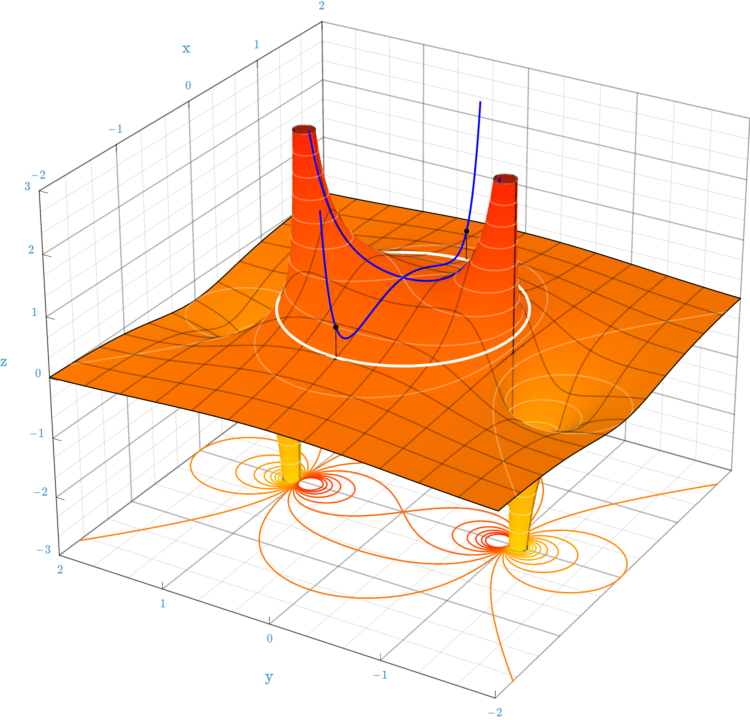
\includegraphics[width=4.5cm]{TaylorComplexConv}
% \end{column}
% \end{columns}
\end{definition}
\end{frame}
\begin{frame}
\frametitle{Some non-uniform results}

$$a_m =\frac{f^{(m)}(x_0)}{m!} 
, \,\, f(x) = \sum_{m=0}^\infty a_m(x-x_0)^k \,\ \text{ for } x \in B(x_0,R)
$$
\vfill
\begin{theorem}[Pour-El, Richards, Ko, Friedman, M\"uller (1987/1989)]
$f$ is (polytime) computable iff $(a_m)_{m \in \N}$ is.
\end{theorem}
 \onslide<2->{
From that polynomial time computability of the derivative and the anti-derivative of a function follows immediately.
}
\end{frame}
\begin{frame}
\frametitle{Some non-uniform results}
$$a_m =\frac{f^{(m)}(0)}{m!} 
, \,\, f(x) = \sum_{m=0}^\infty a_mx^k \,\ \text{ for } x \in B(0,R)
$$
\vfill
\begin{theorem}[M\"uller (1995)]
\begin{itemize}
\item The operator $f \to (a_m)_{m \in \N}$ is not computable.
\item The evaluation operator $((a_m)_{m \in \N},x) \to f(x) $ is not computable.
\end{itemize}
\end{theorem}
\pause
However, if we supply some additional (discrete) information those operators become computable.
\end{frame}
